\usetikzlibrary{shapes, positioning, arrows.meta, shadows}

\begin{figure}[h]
    \centering
    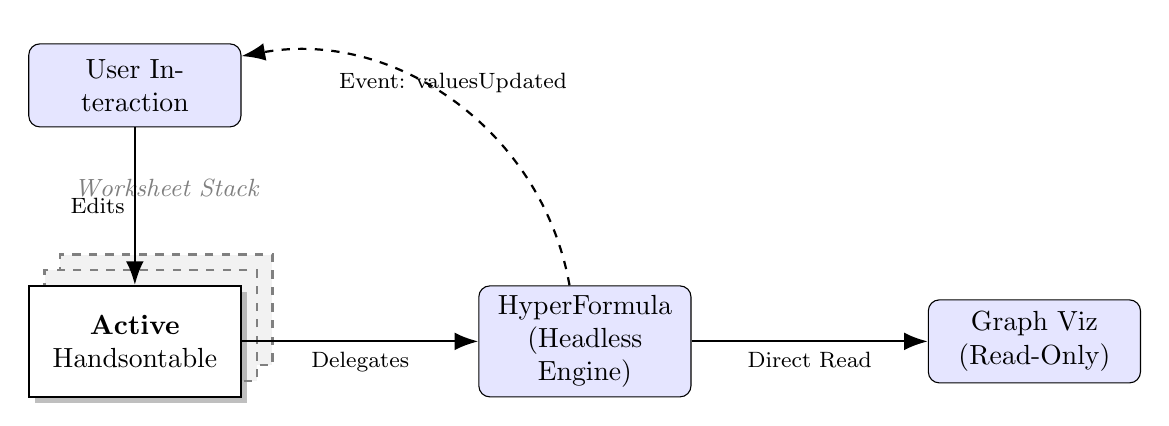
\begin{tikzpicture}[
        node distance=2cm,
        auto,
        % Style for the active (front) sheet
        activeSheet/.style={
            rectangle, draw=black, thick, fill=white, 
            text width=7em, minimum height=4em, 
            text centered, drop shadow
        },
        % Style for inactive (background) sheets
        inactiveSheet/.style={
            rectangle, draw=gray, dashed, thick, fill=gray!10, 
            text width=7em, minimum height=4em, 
            text centered 
        },
        % Standard block style
        block/.style={
            rectangle, draw, fill=blue!10, 
            text width=7em, text centered, rounded corners, minimum height=3em
        },
        line/.style={draw, -{Latex[length=3mm]}, thick}
    ]

        % --- Nodes ---

        % 1. The Stacked Datatables
        % We draw them back-to-front so they overlap correctly
        
        % Inactive Sheet (Back)
        \node [inactiveSheet] (sheet3) at (0.4, 0.4) {};
        
        % Inactive Sheet (Middle)
        \node [inactiveSheet] (sheet2) at (0.2, 0.2) {};
        
        % Active Sheet (Front)
        \node [activeSheet] (sheet1) at (0, 0) {\textbf{Active}\\Handsontable};
        
        % Label for the stack
        \node [above=0.6cm of sheet3, font=\small\itshape, color=gray] {Worksheet Stack};


        % 2. The Other Components
        \node [block, above=2cm of sheet1] (user) {User Interaction};
        \node [block, right=3cm of sheet1] (engine) {HyperFormula\\(Headless Engine)};
        \node [block, right=3cm of engine] (graph) {Graph Viz\\(Read-Only)};


        % --- Edges (The Flow) ---

        % User writes to the ACTIVE sheet only
        \path [line] (user) -- node[left, font=\footnotesize] {Edits} (sheet1);

        % Active sheet delegates to Engine
        \path [line] (sheet1) -- node[below, font=\footnotesize] {Delegates} (engine);

        % Engine updates Graph
        \path [line] (engine) -- node[below, font=\footnotesize] {Direct Read} (graph);

        % (Optional) Feedback loop from Engine to User/UI
        \path [line, dashed, bend right=45] (engine) to node[above, font=\footnotesize] {Event: valuesUpdated} (user);

    \end{tikzpicture}
    \caption{The asymmetric data flow. User edits are routed strictly through the active Handsontable component (foreground), while inactive sheets (background, dashed) remain dormant. The engine updates the graph directly.}
    \label{fig:stacked_flow}
\end{figure}